
\chapter{Finite volume methods}
\label{app:finite}

The aim of this appendix is to explain qualitatively the numerical methods we used during this internship.  Readers looking for a more rigorous - but longer! - presentation of such methods can read \cite{leveque}. 

For the sake of simplicity, we will focus on the one-dimensional conservation law:
\begin{equation}
	\p{}{t} u(t,x) + \p{}{x} f(u(t,x)) = 0
\end{equation}
where $f$ is called the flux function, and where $u(t,x)$ is the unknown solution of the equation we seek to approach numerically. Of course, for us this unknown function is the concentration $\phi$, but it can be another quantity in the general case. Historically, finite volume methods were developed to solve problem from gas dynamics, hence the use of the conventional letter $u$ to label the solution, which in this context is the gas velocity. 

\section{Finite volumes}

The idea of finite volume methods is to discretise the physical -here one-dimensional- space into small volume elements called cells. 
Each cell hold two bits of information: the approximate value of the solution inside the cell, and the approximate value of the flux at each edge of the cell. Cells are usually rectangular, but it is of course not a requirement.
We will also discretise time in small intervals $\Delta T$ called time steps. 

\begin{figure}[htp]
\centering
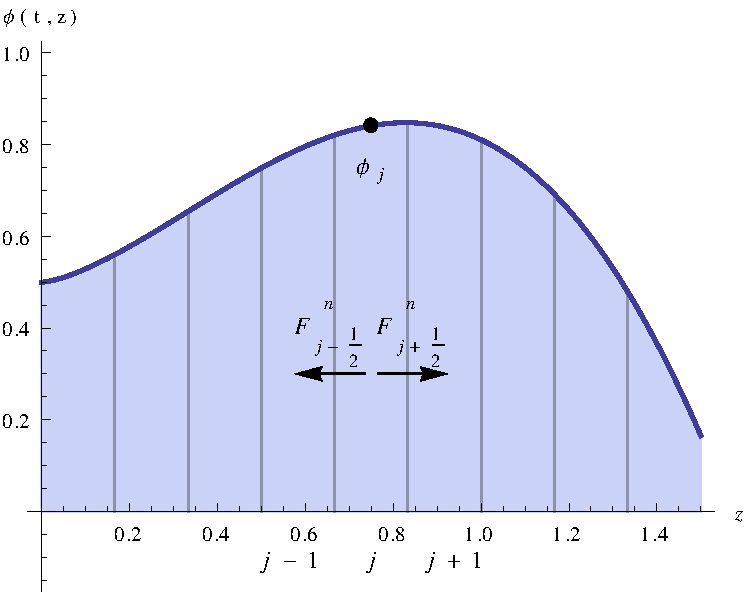
\includegraphics[scale=0.65]{/home/nicolas/git/reports/M1/vector/conservative.pdf}
\caption{$x \rightarrow u(t,x)$ and its discretisation.}
\label{}
\end{figure}

We will call  $u_j^n$ the approximate value of the $u$ function at cell number $j$ after $n$ time steps. We will call the fluxes at the right and left edges of this cell $F_{j+1/2}^n$ and $F_{j-1/2}^n$\footnote{Note that by convention the subscript $j+1/2$ ( $j-1/2$) denote the value of a quantity at the right (left) $j^{\text{th}}$ cell edge.}.

What we want to do is combine these different quantities to create a numerical scheme. The simplest scheme on can think of is obtained replacing derivatives in the conservation by finite differences:
\begin{equation}
	\frac{u^{n+1}_j - u^n_j}{\Delta T} + \frac{f(u^n_{j+1}) - f(u^n_j)}{\Delta x} = 0
\end{equation} 
This scheme involves the cell at position $j$, its right neighbour at $j+1$, but not its left neighbour at $j-1$. This asymmetry between left and right can be an advantage in particular situations, for example if we know that $u$ is advected from left to right. To get rid of this asymmetry and produce a more generally adapted scheme, we can use central differencing:
\begin{equation}
	\frac{u^{n+1}_j - u^n_j}{\Delta T} + \frac{f(u^n_{j+1}) - f(u^n_{j-1})}{2\Delta x} = 0
\end{equation}
However one can show that this scheme is unstable. The simplest generally adapted and stable scheme has been proposed for the first time by Lax and Friedrichs  in \cite{lxf}.
\section{The Lax and Friedrichs scheme}

To get the Lax and Friedrichs scheme from the above equation, we simply replace $u^n_j$ by the mean value over the left and right cells:
\begin{equation}
		\frac{u^{n+1}_j - \frac{  u^n_{j+1} + u^n_{j-1}  }{ 2 } }{\Delta T} + \frac{f(u^n_{j+1}) - f(u^n_{j-1})}{2\Delta x} = 0
\end{equation}
It can be shown that this scheme is stable\footnote{If the so-called Courant-Friedrich-Levy condition is statisfied. Essentially, the ratio of the spatial and temporal discretisation $\Delta x/ \Delta t$ must be chosen greater than the local advection speed.}. Rearranging the different terms, we can write the scheme in \textit{conservative form}:
\begin{equation}
	u^{n+1}_j = u^n_j - \frac{\Delta t}{\Delta x} \left( F^n_{j+1/2}  - F^n_{j+1/2} \right) 
\end{equation}
with
\begin{equation}
	F^n_{j+1/2} = \frac{1}{2} \left( f(u^n_{j+1}) + f(u^n_{j}) \right) - \frac{1}{2} \frac{\Delta x}{\Delta t} \left( u^n_{j+1} - u^n_{j-1} \right)
\end{equation}
The numerical fluxes $F^n_{j+1/2}$ and $F^n_{j-1/2}$ are numerical approximations of the real flux of $u$ at the edges of cell number $j$.
The Lax and Friedrichts scheme is only first-order accurate. To have a better accuracy, one can find better numerical approximations $F^n_{j \pm 1/2}$ of the flux. 

\section{The Kurganov and Tadmor scheme}

The scheme elaborated by Kurganov and Tadmor (cf \cite{KT}) can be seen as a modified version of the Lax and Friedrichs scheme approximating better the flux function. 
The idea is to evaluate numerically the value of $u$ at the edges of the cell to gain accuracy. For example the value at the right edge of cell number $j$, which we call $u^n_{j+1/2}$ accordingly to our notation, will be computed using
\begin{equation}
	u^n_{j+1/2} = u^n_j + \frac{\Delta X}{2}  \p{}{x} u^n_j
\end{equation}
where the partial derivative is computed using a finite difference formula.
Note that unless our finite differences are perfectly accurate, $u^n_{j+1/2} \neq u^n_{(j+1) - 1/2}$!
The numerical flux is now
\begin{equation}
	F^n_{j+1/2} = \frac{1}{2} \left( f(u^n_{j+1/2}) + f(u^n_{(j+1)-1/2}) \right) - \frac{1}{2} | a^n_{j+1/2} | \left( u^n_{(j+1)-1/2} - u^n_{j+1/2} \right)
\end{equation}
Note that the term $\Delta x/\Delta t$ has been replaced by the local advection speed $| a_{j+1/2}^n|$. This also plays a key role in ensuring the accuracy of the scheme.

The Kurganov and Tadmor scheme is remarkably simple, accurate and stable. 
If we chose a correct finite difference formula to compute the derivatives appearing in the edges values of $u$, the scheme can be shown to be second order accurate. That means that shocks, frequently appearing in the solutions of conservation laws, will be well resolved. It also exhibits the important \textit{total variation diminishing property}, which ensures that no oscillations will appear near the shocks. 
